%% OLD VERSION of a part of Stellarium User Guide
%% History:
%% 2016-04-24 Replaced by new chapter. 
%% State: Defunct.

\chapter{Landscapes}\label{customising-landscapes}
\label{ch:landscapes}

Stellarium comes with a selection of panorama landscapes which try to
link the sky with the observer's surrounding and thus create a more
immersive feeling.  It is possible to create your own landscapes for
Stellarium, this is described in
section~\ref{sec:landscapes:customizing}. 

\section{Landscape Types}
\label{sec:landscapes:types}


There are four types of landscape:

\begin{itemize}
\item
  \textbf{Polygonal Method} Using a text file with azimuths/altitudes.
\item
  \textbf{Single Fish-eye Method} Using a fish-eye panorama image.
\item
  \textbf{Single Spherical Method} Using a spherical panorama image.
\item
  \textbf{Multiple Image Method} (\textbf{also called ``old style''
  landscapes}) Using a series of images split from a 360$\degree$ ``strip''
  panorama image + a ground image.
\end{itemize}

Each landscape has its own sub-directory in
\texttt{\textless{}user\ directory\textgreater{}/landscapes} or
\texttt{\textless{}installation\ directory\textgreater{}/landscapes}.
The name of the sub-directory is called the \emph{landscape ID}. The
sub-directory must contain a file called \texttt{landscape.ini} which
describes the landscape type, texture filenames and other data. Texture
files for a landscape should by put in the same directory as the
\texttt{landscape.ini} file, although if they are not found there they
will be searched for in the \texttt{.../textures} directory, allowing
shared files for common textures such as the generic fog texture.

For example, the \emph{Moon} landscape that is provided with Stellarium
has the following files:

\texttt{.../landscapes/moon/landscape.ini}\\
\texttt{.../landscapes/moon/apollo17.png}

The \texttt{landscape.ini} file must contain a section called
\texttt{{[}landscape{]}}, which contains the details necessary to render
the landscape (which vary, depending on the type of the landscape).

There is also an optional \texttt{{[}location{]}} section which is used
to tell Stellarium where the landscape is in the solar system. If the
\texttt{{[}location{]}} section exists, Stellarium can automatically
adjust the location and observing conditions of the observer to match
the landscape.

\subsection{Polygonal Landscape}\label{polygonal-line-method}

This is the technically simplest of the landscapes, but may be used to
describe accurately measured horizon lines. The file that encodes
horizon altitudes can also be used in all other landscape types. If
present there, it will be used to define object visibility (instead of
the opacity of the landscape photo textures) and, if
\texttt{horizon\_line\_color} is defined, will be plotted.

There is a small caveat: Sometimes, there may appear vertical lines from
some corners towards the zenith or the mathematical horizon, e.g. if
there is a vertex including azimuth 0 or 180. If this irritates you,
just offset this azimuth minimally (e.g., 180.00001).

The \texttt{landscape.ini} file for a polygonal type landscape looks
like this (this example is based on the Geneve landscape which was
borrowed from Cartes du Ciel and comes with Stellarium):

\begin{config}
\texttt{{[}landscape{]}}\\
\texttt{name~=~Geneve}\\
\texttt{type~=~polygonal}\\
\texttt{author~=~Georg~Zotti;~Horizon~definition~by~Patrick~Chevalley}\\
\texttt{description~=~Horizon~line~of~Geneve.~Demonstrates~compatibility~with~horizon~descriptions~from~~Cartes~du~Ciel.}\\
\texttt{polygonal\_horizon\_list~=~horizon\_Geneve.txt}\\
\texttt{polygonal\_angle\_rotatez~=~0}\\
\texttt{ground\_color~=~.15,.45,.45}\\
\texttt{horizon\_line\_color~=~~.75,.45,.45}
\end{config}

Where:

\begin{itemize}
\item
  \textbf{name} is what appears in the landscape tab of the
  configuration window.
\item
  \textbf{type} identifies the method used for this landscape.
  ``polygonal'' in this case.
\item
  \textbf{author} lists the author(s) responsible for images and
  composition.
\item
  \textbf{description} gives a short description visible in the
  selection panel. The text will be superseded by optional
  \texttt{description.\&lt;lang\&gt;.utf8} files.
\item
  \textbf{polygonal\_horizon\_list} is the name of the horizon data file
  for this landscape.
\item
  \textbf{polygonal\_horizon\_list\_mode} (optional) the two first
  columns in the list are numbers: azimuth and altitude or zenith
  distance, in either degrees or radians or gradians(gon). The value
  must be one of
  \texttt{azDeg\_altDeg\textbar{}azDeg\_zdDeg\textbar{}azRad\_altRad\textbar{}azRad\_zdRad\textbar{}azGrad\_altGrad\textbar{}azGrad\_zdGrad}.
  Default: azDeg\_altDeg
\item
  \textbf{polygonal\_angle\_rotatez} (optional, default=0) Angle
  (degrees) to adjust azimuth. This may be used to apply a (usually)
  small offset rotation, e.g. when you have measured the horizon in a
  grid-based coordinate system like UTM and have to compensate for the
  meridian convergence.
\item
  \textbf{ground\_color} (optional, default=``0,0,0'', i.e., black)
  Color for the area below the horizon line. Each R,G,B component is a
  float within 0..1.
\item
  \textbf{horizon\_line\_color} (optional, default: invisible) used to
  draw a polygonal horizon line. Each R,G,B component is a float within
  0..1.
\item
  \textbf{minimal\_brightness} (optional, default=-1, i.e. use preset
  landscape/minimal\_brightness from global \texttt{config.ini}) Some
  minimum brightness to keep landscape visible.
\item
  \textbf{minimal\_altitude} (optional, default=-2) Some sky elements,
  e.g. stars, are not drawn below this altitude. Under certain
  circumstances you may want to specify something else here. (since
  V0.14)
\end{itemize}

\subsection{Single Fish-eye Landscape}\label{single-fish-eye-method}

The \emph{Trees} landscape that is provided with Stellarium is an
example of the single fish-eye method, and provides a good illustration.
The centre of the image is the spot directly above the observer (the
zenith). The point below the observer (the nadir) becomes a circle that
just touches the edges of the image. The remaining areas of the image
(the corners outside the circle) are not used.

The image file should be saved in PNG format with alpha transparency.
Wherever the image is transparent is where Stellarium will render the
sky.

The \texttt{landscape.ini} file for a fish-eye type landscape looks like
this (this example is based on the Trees landscape which comes with
Stellarium):

\begin{config}
\texttt{{[}landscape{]}}\\
\texttt{name~=~Trees}\\
\texttt{type~=~fisheye}\\
\texttt{author~=~Robert~Spearman.~Light~pollution~image:~Georg~Zotti}\\
\texttt{description~=~Trees~in~Greenlake~Park,~Seattle}\\
\texttt{maptex~=~trees\_512.png}\\
\texttt{maptex\_illum~=~trees\_illum\_512.png}\\
\texttt{maptex\_fog~=~trees\_fog\_512.png}\\
\texttt{texturefov~=~210}\\
\texttt{angle\_rotatez~=~17}\\
\texttt{tesselate\_rows~=~28}\\
\texttt{tesselate\_cols~=~60}
\end{config}

Where:

\begin{itemize}
\item
  \textbf{name} is what appears in the landscape tab of the
  configuration window.
\item
  \textbf{type} identifies the method used for this landscape.
  ``fisheye'' in this case.
\item
  \textbf{author} lists the author(s) responsible for images and
  composition.
\item
  \textbf{description} gives a short description visible in the
  selection panel. The text will be superseded by optional
  \texttt{description.\&lt;lang\&gt;.utf8} files.
\item
  \textbf{maptex} is the name of the image file for this landscape.
\item
  \textbf{maptex\_fog} (optional) is the name of the fog image file for
  this landscape.
\item
  \textbf{maptex\_illum} (optional) is the name of the nocturnal
  illumination/light pollution image file for this landscape.
\item
  \textbf{texturefov} is the field of view that the image covers in
  degrees.
\item
  \textbf{angle\_rotatez} (optional) Angle (degrees) to adjust azimuth.
\item
  \textbf{tesselate\_rows} (optional, default=20) If straight edges in
  your landscape appear broken, try increasing.
\item
  \textbf{tesselate\_cols} (optional, default=40) If straight edges in
  your landscape appear broken, try increasing.
\item
  \textbf{polygonal\_horizon\_list} (optional) is the name of the
  (measured) horizon data file for this landscape.
\item
  \textbf{polygonal\_horizon\_list\_mode} (optional) the two first
  columns in the list are numbers: azimuth and altitude or zenith
  distance, in either degrees or radians or gradians(gon). The value
  must be one of
  \texttt{azDeg\_altDeg \textbar{} azDeg\_zdDeg \textbar{} azRad\_altRad \textbar{} azRad\_zdRad \textbar{} azGrad\_altGrad \textbar{} azGrad\_zdGrad}.
  Default: \texttt{azDeg\_altDeg}
\item
  \textbf{polygonal\_angle\_rotatez} (optional, default=0) Angle
  (degrees) to adjust azimuth. This may be used to apply a (usually)
  small offset rotation, e.g. when you have measured the horizon in a
  grid-based coordinate system like UTM and have to compensate for the
  meridian convergence.
\item
  \textbf{horizon\_line\_color} (optional, default: invisible) used to
  draw a polygonal horizon line.
\item
  \textbf{minimal\_brightness} (optional, default=-1, i.e. use preset
  landscape/minimal\_brightness from global \texttt{config.ini}) Some
  minimum brightness to keep landscape visible.
\item
  \textbf{minimal\_altitude} (optional, default=-2) Some sky elements,
  e.g. stars, are not drawn below this altitude. Under certain
  circumstances you may want to specify something else here. (since
  V0.14)
\end{itemize}

\subsection{Single Panorama Landscape}\label{single-panorama-method}

This method uses a more usual type of panorama - the kind which is
produced directly from software such as \emph{autostitch} or Hugin
(http://hugin.sourceforge.net/). The panorama file should be copied into
the
\texttt{\textless{}config\ root\textgreater{}/landscapes/\textless{}landscape\_id\textgreater{}}
directory, and a \texttt{landscape.ini} file created. The \emph{Moon}
landscape which comes with Stellarium provides a minimal example of the
contents of a landscape.ini file for a spherical type landscape:

\begin{config}
\texttt{{[}landscape{]}}\\
\texttt{name~=~Moon}\\
\texttt{type~=~spherical}\\
\texttt{maptex~=~apollo17.png}
\end{config}

A more elaborate example is found with the \emph{Grossmugl} landscape:

\begin{config}
\texttt{{[}landscape{]}}\\
\texttt{name~=~Grossmugl}\\
\texttt{type~=~spherical}\\
\texttt{author~=~Guenther~Wuchterl,~Kuffner-Sternwarte.at;~Lightscape:~Georg~Zotti}\\
\texttt{description~=~Field~near~Leeberg,~Grossmugl~(Riesentumulus),~Austria~-~Primary~Observing~Spot~of~the~Grossmugl~Starlight~Oasis~-~}\url{http://starlightoasis.org}}\\
\texttt{maptex~=~grossmugl\_leeberg\_crop11.25.png}\\
\texttt{maptex\_top=11.25~}\\
\texttt{maptex\_fog~=~grossmugl\_leeberg\_fog\_crop22.5.png}\\
\texttt{maptex\_fog\_top~=~22.5}\\
\texttt{maptex\_fog\_bottom~=~-22.5}\\
\texttt{maptex\_illum~=~grossmugl\_leeberg\_illum\_crop0.png}\\
\texttt{maptex\_illum\_bottom~=~0}\\
\texttt{angle\_rotatez=-89.1}\\
\texttt{minimal\_brightness~=~0.0075}\\
\texttt{polygonal\_horizon\_list~=~horizon\_grossmugl.txt}\\
\texttt{polygonal\_angle\_rotatez=0}\\
\texttt{horizon\_line\_color~=~~.75,.45,.45}\\
\texttt{minimal\_altitude~=~-1}
\end{config}

Where:

\begin{itemize}
\item
  \textbf{name} is what appears in the landscape tab of the
  configuration window.
\item
  \textbf{type} identifies the method used for this landscape.
  ``spherical'' in this case.
\item
  \textbf{author} lists the author(s) responsible for images and
  composition.
\item
  \textbf{description} gives a short description visible in the
  selection panel. The text will be superseded by optional
  \texttt{description.\&lt;lang\&gt;.utf8} files.
\item
  \textbf{maptex} is the name of the image file for this landscape.
\item
  \textbf{maptex\_top} (optional; default=90) is the altitude angle of
  the top edge.
\item
  \textbf{maptex\_bottom} (optional; default=-90) is the altitude angle
  of the bottom edge. Usually you will not require this, or else there
  will be a hole at your feet. ;-)
\item
  \textbf{maptex\_fog} (optional; default: no fog) is the name of the
  fog image file for this landscape.
\item
  \textbf{maptex\_fog\_top} (optional; default=90) is the altitude angle
  of the top edge of the fog texture. Useful to crop away parts of the
  image to conserve texture memory.
\item
  \textbf{maptex\_fog\_bottom} (optional; default=-90) is the altitude
  angle of the bottom edge.
\item
  \textbf{maptex\_illum} (optional; default: no illumination layer) is
  the name of the nocturnal illumination/light pollution image file for
  this landscape.
\item
  \textbf{maptex\_illum\_top} (optional; default=90) is the altitude
  angle of the top edge, if you have light pollution only close to the
  horizon.
\item
  \textbf{maptex\_illum\_bottom} (optional; default=-90) is the altitude
  angle of the bottom edge.
\item
  \textbf{angle\_rotatez} (optional, default=0) Angle (degrees) to
  adjust azimuth. If 0, the left/right edge is due east.
\item
  \textbf{tesselate\_rows} (optional, default=20) If straight edges in
  your landscape appear broken, try increasing. This is the number of
  rows for the maptex. Fog and illumination textures will have a similar
  vertical angle.
\item
  \textbf{tesselate\_cols} (optional, default=40) If straight edges in
  your landscape appear broken, try increasing.
\item
  \textbf{polygonal\_horizon\_list} (optional) is the name of the
  (measured) horizon data file for this landscape. Can be used to query
  horizon transparency (for accurate object rising/setting times)
\item
  \textbf{polygonal\_horizon\_list\_mode} (optional) the two first
  columns in the list are numbers: azimuth and altitude or zenith
  distance, in either degrees or radians or gradians(gon). The value
  must be one of
  \texttt{azDeg\_altDeg\textbar{}azDeg\_zdDeg\textbar{}azRad\_altRad\textbar{}azRad\_zdRad\textbar{}azGrad\_altGrad\textbar{}azGrad\_zdGrad}.
  Default: \texttt{azDeg\_altDeg}
\item
  \textbf{polygonal\_angle\_rotatez} (optional, default=0) Angle
  (degrees) to adjust azimuth. This may be used to apply a (usually)
  small offset rotation, e.g. when you have measured the horizon in a
  grid-based coordinate system like UTM and have to compensate for the
  meridian convergence.
\item
  \textbf{horizon\_line\_color} (optional, default: invisible) used to
  draw a polygonal horizon line.
\item
  \textbf{minimal\_brightness} (optional, default=-1, i.e. use preset
  landscape/minimal\_brightness from global config.ini) Some minimum
  brightness to keep landscape visible.
\item
  \textbf{minimal\_altitude} (optional, default=-2) Some sky elements,
  e.g. stars, are not drawn below this altitude. Under certain
  circumstances (e.g. for space station panoramas where you may have sky
  below your feet, or for deep valleys/high mountains for efficiency,
  you may want to specify something else here. (since V0.14)
\end{itemize}

To save texture memory, since V0.13 you can trim away the transparent
sky and define the angle \textbf{maptex\_top}. Likewise,
\textbf{fogtex\_top}, \textbf{fogtex\_bottom},
\textbf{maptex\_illum\_top} and \textbf{maptex\_illum\_top}. You should
then stretch the texture to a full power of 2, like 4096x1024. The
easiest method to create perfectly aligned fog and illumination layers
is with an image editor that supports layers like the GIMP or Photoshop.
Fog and Light images should have black background.

\subsection{Multiple Image Landscape}\label{multiple-image-method}

The multiple image method works by having a 360 panorama of the horizon
(without wasting too much texture memory with the sky) split into a
number of smaller ``side textures'', and a separate ``ground texture''.
This has the advantage over the single image method that the detail
level of the horizon can be increased further without ending up with a
single very large image file, so this is usable for either very
high-resolution panoramas or for older hardware. The ground texture can
be a lower resolution than the panorama images. Memory usage may be more
efficient because there are no unused texture parts like the corners of
the texture file in the fish-eye method. It is even possible to repeat
the horizon several times (for purely decorative purpose). The side
textures are indeed mapped onto curved (spherical ring or cylinder)
walls, not flat sides as shown here.

\begin{figure}[h]
\centering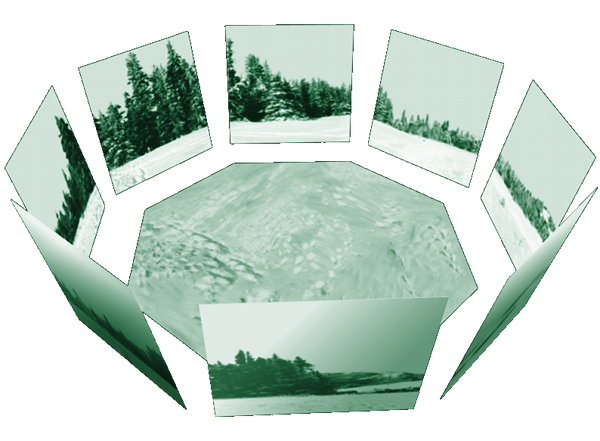
\includegraphics[scale=0.7]{faq_landscape}
%\caption{Figure caption}
\end{figure}

On the negative side, it is more difficult to create this type of
landscape - merging the ground texture with the side textures can prove
tricky. The contents of the \texttt{landscape.ini} file for this
landscape type is also somewhat more complicated than for other
landscape types. Here is the \texttt{landscape.ini} file which describes
the Guereins landscape:

\begin{config}
\texttt{{[}landscape{]}}\\
\texttt{name~=~Guereins}\\
\texttt{type~=~old\_style}\\
\texttt{author~=~Fabien~Chéreau}\\
\texttt{description~=~Guéreins~is~a~small~french~village...}\\
\texttt{nbsidetex~=~8}\\
\texttt{tex0~=~guereins4.png}\\
\texttt{tex1~=~guereins5.png}\\
\texttt{tex2~=~guereins6.png}\\
\texttt{tex3~=~guereins7.png}\\
\texttt{tex4~=~guereins8.png}\\
\texttt{light4~=~guereins8-lgt.png}\\
\texttt{tex5~=~guereins1.png}\\
\texttt{tex6~=~guereins2.png}\\
\texttt{tex7~=~guereins3.png}\\
\texttt{nbside~=~8}\\
\texttt{side0~=~tex0:0:0.005:1:1}\\
\texttt{side1~=~tex1:0:0.005:1:1}\\
\texttt{side2~=~tex2:0:0.005:1:1}\\
\texttt{side3~=~tex3:0:0.005:1:1}\\
\texttt{side4~=~tex4:0:0.005:1:1}\\
\texttt{side5~=~tex5:0:0.005:1:1}\\
\texttt{side6~=~tex6:0:0.005:1:1}\\
\texttt{side7~=~tex7:0:0.005:1:1}\\
\texttt{groundtex~=~guereinsb.png}\\
\texttt{fogtex~=~fog.png}\\
\texttt{nb\_decor\_repeat~=~1}\\
\texttt{decor\_alt\_angle~=~40}\\
\texttt{decor\_angle\_shift~=~-22}\\
\texttt{decor\_angle\_rotatez~=~0}\\
\texttt{ground\_angle\_shift~=~-22}\\
\texttt{ground\_angle\_rotatez~=~45}\\
\texttt{fog\_alt\_angle~=~20}\\
\texttt{fog\_angle\_shift~=~-3}\\
\texttt{draw\_ground\_first~=~1}
\end{config}

Where:

\begin{itemize}
\item
  \textbf{name} is the name that will appear in the landscape tab of the
  configuration window for this landscape
\item
  \textbf{type} should be ``old\_style'' for the multiple image method.
\item
  \textbf{author} lists the author(s) responsible for images and
  composition.
\item
  \textbf{description} gives a short description visible in the
  selection panel. The text will be superseded by optional
  description..utf8 files.
\item
  \textbf{nbsidetex} is the number of side textures for the landscape.
\item
  \textbf{tex0 ... tex} are the side texture file names. These should
  exist in the \texttt{.../textures/landscapes} directory in PNG format.
\item
  \textbf{light0 ... light} are optional textures. If they exist, they
  are used as overlays on top of the respective
  tex\textless{}...\textgreater{} files and represent nocturnal
  illumination, e.g. street lamps, lit windows, red dots on towers, sky
  glow by city light pollution, ... Empty panels don't have to exist. If
  you need your light pollution higher in the sky, you must use a
  spherical or fisheye landscape. (New feature, V0.13.1)
\item
  \textbf{nbside} is the number of side textures
\item
  \textbf{side0 ... side} are the descriptions of how the side textures
  should be arranged in the program. Each description contains five
  fields separated by colon characters (:). The first field is the ID of
  the texture (e.g. tex0), the remaining fields are the texture
  coordinates (x0:y0:x1:y1) used to place the texture in the scene. If
  you want to use all of the image, this will just be \texttt{0:0:1:1}.
\item
  \textbf{groundtex} is the name of the ground texture file. (This could
  also be a diagram e.g. indicating the mountain peaks!)
\item
  \textbf{ground} {[}NO LONGER USED{]} used to be the description of the
  projection of the ground texture in the scene.
\item
  \textbf{fogtex} is the name of the texture file for fog in this
  landscape. Note that for this landscape, accurate overlay of fog and
  landscape is only done if \texttt{calibrated=true} and
  \texttt{tan\_mode=true}.
\item
  \textbf{fog} {[}NO LONGER USED{]} used to be the description of the
  projection of the fog texture in the scene.
\item
  \textbf{nb\_decor\_repeat} is the number of times to repeat the side
  textures in the 360 panorama. (Photo panoramas should have ``1'' here)
\item
  \textbf{decor\_alt\_angle} (degrees) is the vertical angular size of
  the textures (i.e. how high they go into the sky).
\item
  \textbf{decor\_angle\_shift} (degrees) vertical angular offset of the
  scenery textures, at which height are the side textures placed.
\item
  \textbf{decor\_angle\_rotatez} (degrees) angular rotation of the
  scenery around the vertical axis. This is handy for rotating the
  landscape so North is in the correct direction.
\item
  \textbf{ground\_angle\_shift} (degrees) vertical angular offset of the
  ground texture, at which height the ground texture is placed.
\item
  \textbf{ground\_angle\_rotatez} (degrees) angular rotation of the
  ground texture around the vertical axis. When the sides are rotated,
  the ground texture may need to be rotated as well to match up with the
  sides.
\item
  \textbf{fog\_alt\_angle} (degrees) vertical angular size of the fog
  cylinder - how fog looks. Accurate vertical size requires
  \texttt{calibrated=true}.
\item
  \textbf{fog\_angle\_shift} (degrees) vertical angular offset of the
  fog texture - at what height is it drawn. Accurate vertical placement
  requires \texttt{calibrated=true}.
\item
  \textbf{draw\_ground\_first} if 1 the ground is drawn in front of the
  scenery, i.e. the side textures will overlap over the ground texture.
\item
  \textbf{calibrated} (optional, not used in this file). New since
  0.10.6: Only if true, decor\_alt\_angle etc. really work as documented
  above. The (buggy) old code was left to work with the landscapes
  already existing.
\item
  \textbf{tan\_mode} (optional, not used in this file). If true, the
  panorama image must be in in cylindrical, not equirectangular
  projection. Finding \texttt{decor\_alt\_angle} and
  \texttt{decor\_angle\_shift} may be a bit more difficult with this,
  but now (V0.13) works also with calibrated. A fog image created as
  overlay on the pano will be perfectly placed.
\item
  \textbf{decor\_angle\_rotatez} angular rotation of the scenery around
  the vertical axis. This is handy for rotating the landscape so North
  is in the correct direction. If 0, the left edge of \texttt{tex0} is
  due east.
\item
  \textbf{ground\_angle\_shift} vertical angular offset of the ground
  texture, at which height the ground texture is placed. Values above
  -10 are not recommended for non-photographic content due to high
  distortion.
\item
  \textbf{ground\_angle\_rotatez} angular rotation of the ground texture
  around the vertical axis. When the sides are rotated, the ground
  texture may need to be rotated as well to match up with the sides. If
  0, east is up. if North is up in your image, set this to 90.
\item
  \textbf{fog\_alt\_angle} vertical angular size of the fog texture -
  how fog looks.
\item
  \textbf{fog\_angle\_shift} vertical angular offset of the fog texture
  - at what height is it drawn.
\item
  \textbf{draw\_ground\_first} if 1 the ground is drawn before the
  sides, i.e. the side textures may overlap the ground texture if
  \texttt{ground\_angle\_shift\ \&gt;\ decor\_angle\_shift}.
\item
  \textbf{polygonal\_horizon\_list} (optional) is the name of the
  (measured) horizon data file for this landscape. Can be used to query
  horizon transparency (for accurate object rising/setting times)
\item
  \textbf{polygonal\_horizon\_list\_mode} (optional) the two first
  columns in the list are numbers: azimuth and altitude or zenith
  distance, in either degrees or radians or gradians(gon). The value
  must be one of
  azDeg\_altDeg\textbar{}azDeg\_zdDeg\textbar{}azRad\_altRad\textbar{}azRad\_zdRad\textbar{}azGrad\_altGrad\textbar{}azGrad\_zdGrad.
  Default: azDeg\_altDeg
\item
  \textbf{polygonal\_angle\_rotatez} (optional, default=0) Angle
  (degrees) to adjust azimuth. This may be used to apply a (usually)
  small offset rotation, e.g. when you have measured the horizon in a
  grid-based coordinate system like UTM and have to compensate for the
  meridian convergence.
\item
  \textbf{horizon\_line\_color} (optional, default: invisible) used to
  draw a polygonal horizon line.
\item
  \textbf{minimal\_brightness} (optional, default=-1, i.e. use preset
  landscape/minimal\_brightness from global config.ini) Some minimum
  brightness to keep landscape visible.
\item
  \textbf{minimal\_altitude} (optional, default=-2) Some sky elements,
  e.g. stars, are not drawn below this altitude. Under certain
  circumstances you may want to specify something else here. (since
  V0.14)
\end{itemize}

\subsection{landscape.ini {[}location{]} section}\label{landscape.ini-location-section}

An example location section:

\begin{config}
\texttt{{[}location{]}}\\
\texttt{planet~=~Earth}\\
\texttt{latitude~=~+48d10'9.707"}\\
\texttt{longitude~=~+11d36'32.508"}\\
\texttt{altitude~=~83}\\
\texttt{light\_pollution=3}\\
\texttt{atmospheric\_extinction\_coefficient=0.2}\\
\texttt{atmospheric\_temperature=10}\\
\texttt{atmospheric\_pressure=-1}
\end{config}

Where:

\begin{description}
\item[planet] Is the English name of the solar system body for the
  landscape.
\item[latitude] Is the latitude of site of the landscape in degrees,
  minutes and seconds. Positive values represent North of the equator,
  negative values South of the equator.
\item[longitude] Is the longitude of site of the landscape. Positive
  values represent East of the Greenwich Meridian on Earth (or
  equivalent on other bodies), Negative values represent Western
  longitude.
\item[altitude] Is the altitude of the site of the landscape in
  meters.
\item[country] (optional) Name of the country the location is in
\item[state] (optional) Name of the state the location is in
\item[name] (optional) Name of the location
\end{description}

Since 0.11, there are a few more optional parameters that can be loaded
if the according switch is active in the landscape selection panel. If
they are missing, the parameters do not change to defaults.

\begin{description}
\item[light\_pollution] (optional) Light pollution of the site,
  given on the Bortle Scale (1: none ... 9: metropolitan). If negative
  or absent, no change will be made.
\item[atmospheric\_extinction\_coefficient] (optional, no change if
  absent.) Extinction coefficient (mag/airmass) for this site.
\item[atmospheric\_temperature] (optional, no change if absent.)
  Surface air temperature (Degrees Celsius). Used for refraction. . Set
  to -1000 to explicitly declare ``no change''.
\item[atmospheric\_pressure] (optional, no change if absent.)
  Surface air pressure (mbar; would be 1013 for ``normal'' sea-level
  conditions). Used for refraction. Set to -2 to declare ``no change'',
  or -1 to compute from altitude.
\item[display\_fog] (optional, -1/0/1, default=-1) You may want to
  preconfigure setting \textbf{0} for a landscape on the Moon. Set -1 to
  declare ``no change''.
\end{description}

\section{Making a Multi panel Panorama}\label{making-a-multi-panel-panorama}

\begin{figure}[h]
\centering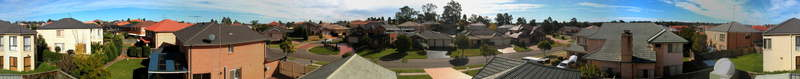
\includegraphics[scale=2.2]{landscape_beaumonthills.jpg}
%\caption{Figure caption}
\end{figure}

This is the only way to get a high resolution panorama and although this
procedure is based on the Microsoft Windows System the basics will apply
to any platform that can run the programs mentioned or similar programs
on the preferred system. If you want a high resolution this is the only
method to use. The first thing needed for a personalised landscape to
superimpose on the horizon display is a 360$\degree$ panorama with a transparent
background. To make this you will need the following:

\begin{itemize}
\item
  A digital camera on a tripod or stable platform
\item
  A program to convert the pictures into a 360$\degree$ panorama
\item
  A program to remove the background and convert the panorama into about
  8 square pictures in PNG format for insertion into Stellarium as the
  sides and if possible a similar square picture of the base you are
  standing on to form the ground. This last requirement is only really
  possible if this area is relatively featureless as the problem of
  knitting a complex base is well nigh impossible.
\item
  Patience. (Maybe a soundproof room so that the swearing wont be heard
  when you press the wrong key and lose an hours work)
\end{itemize}

\subsection{The Camera}\label{the-camera}

Digital cameras are easy and cheaply available these days so whatever
you have should do. One mega-pixel resolution is quite sufficient.

The camera needs to be mounted on a tripod so that reasonably orientated
pictures can be taken. Select a time of day that is quite bright with a
neutral cloudy sky so there will be no shadows and a sky of the same
overall texture. This will make it easier to remove later. The pictures
were all saved in the JPG format which was used as the common format for
all processes up to the removal of the background.

With a camera that takes 4:3 ratio pictures I found 14 evenly spaced
pictures gave the best 360$\degree$ panorama in the program I used to produce
it.

\subsection{Processing into a
Panorama}\label{processing-into-a-panorama}

This is the most complicated part of the process of generating the
panorama. I used two separate programs to do this. Firstly I used The
Gimp to re size the panels to 1024x768 and so make them easier to handle
in the panorama program.

When I had my 14 processed pictures I inserted them into the panorama
program. I first used a program called the Panorama Factory. Version 1.6
is a freebee that works well and can be downloaded from the internet - a
Google search will find it. I later used version 3.4 that is better and
cost about \$40 off the Internet. This program has many options and can
be configured to suit most cameras and can make a seamless 360$\degree$ panorama
in barrel form that will take a highly trained eye to find where the
joins occur.

The resulting panorama was then loaded into The Gimp and trimmed to a
suitable size. Mine ended up 14024 x 1601 pixels. I trimmed the vertical
size to 1024 by cutting back then stretched the 14024 to 14336 pixels,
with almost no distortion, that would allow cutting into 14 1024 x1024
pictures at a later date. If the height of the panorama had been greater
I could have made fewer pictures and so shown more of the foreground.
See figure {[}fig:panorama360{]}.

If you have prominent foreground items like posts wires etc. that occur
in adjacent pictures the panorama program will have difficulty in
discerning them because of the 3D effect and may give double images. I
overcame this by painting out the offending item by cut and paste
between the two pictures. Quite easy with a little practice using the
zoom in facility and I found the MSpaint program the easiest to do this
in.

\begin{figure}[h]
\centering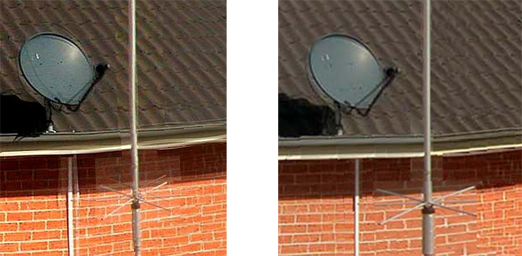
\includegraphics[scale=2.0]{BEAU-3c}
%\caption{Figure caption}
\end{figure}

\subsection{Removing the background to make it
transparent}\label{removing-the-background-to-make-it-transparent}

This is the most complex part of the process and requires a program that
can produce transparency to parts of your picture, commonly called an
alpha channel. Two programs I know of will do this. The very expensive
and sophisticated Adobe Photoshop and a freebee called The Gimp. I used
photoshop to cut the full panorama into 1024 x 1024 textures because it
was the easiest to do accurate cutting but it can be done in TheGimp as
well.

I first used Photoshop to produce the alpha channel because it was the
only way I knew but I now use the GIMP as it is much easier to process
the individual textures than removing the background from the full
panorama.

\begin{enumerate}
\item
  Load the 1st section into TheGimp
\item
  Next create a new empty picture 1024 x 1024 then use the advanced tab
  to make the background color transparency. Copy the original texture
  onto this new picture base so that it exactly fits the frame then
  select layer from the menu and press anchor. This will create a new
  picture with with an alpha channel. By using the select by color and
  lasso etc cut out the parts you don't want this will expose the
  checkerboard background. When you are happy with the removal save the
  texture in *.png format to preserve the alpha layer.
\item
  Do the same with the remaining pictures to make all the components of
  the landscape.
\item
  Make a new directory for the landscape. This should be a sub-directory
  of either the /landscapes or /landscapes directory. The name of the
  directory should be unique to your landscape, and is the landscape ID.
  The convention is to use a single descriptive word in lowercase text,
  for example gueriens. Place your pictures your new directory.
\item
  In your new landscape directory, create a new file called
  landscape.ini file (I used wordpad). Add a line for the
  {[}landscape{]} section. It's probably easiest to copy the
  landscape.ini file for the Gueriens landscape and edit it. Edit the
  name Guereins in every instance to the name you have given your
  landscape. Don't forget to make the number of tex entries agree with
  the number of your pictures. If you haven't made a groundtex picture
  use one of the existing ones from the file or make a square blank
  picture of your own idea. Because I took my pictures from the roof of
  the house I used an edited picture of the roof of my house from Google
  Earth. It was pretty cruddy low resolution but served the purpose.
\item
  Next you need to orientate your picture North with true North. This is
  done roughly by making the arrangement of side1 to siden suit your
  site as close as possible. Now you need to edit the value of
  decor\_angle\_rotatez to move your landscape in azimuth. Edit
  decor\_alt\_angle to move you landscape in altitude to align your
  visible horizon angle. Edit ground\_angle\_rotatez to align your
  ground with the rest of the landscape. Leave the other entries they
  are suitable as is.
\end{enumerate}

After re-starting Stellarium, your landscape will appear in the
landscape folder of the main menu , and can be selected as required.

\section{Making a Spherical Panorama}
\label{making-a-spherical-panorama}

A simpler method of making a panorama is to use the spherical method.
These can be made to create the full panorama using the program
Autostitch. The big advantage of the spherical panorama is that it does
not need a ground panel. However the drawback with the Spherical
panorama is that few computer video cards will reproduce a panorama
larger than 4096 x 2048 pixels and many will not do better than 2048 x
1024 pixels

\begin{figure}[h]
\centering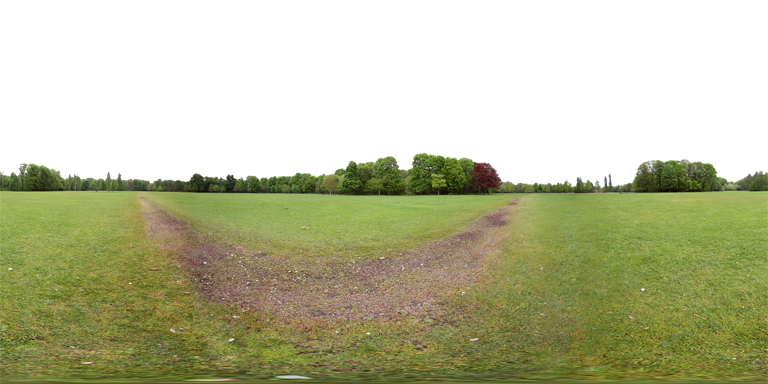
\includegraphics{egarden}
%\caption{Figure caption}
\end{figure}

The Autostitch program is quite easy to use. Make sure your panorama
shots take the ground almost up to your feet and follow the instructions
in the readme file. When the
panorama is finished it will be in *.jpg format. This will need to be
converted to a *.png with transparent background (alpha layer) and have
the sky removed. This can be done in TheGimp as in the multi-panel type.
When the sky is removed make sure you save the landscape in *.png
format.

My computer will only do 2048 by 1024, If I try to load a larger type I
just get a white screen. With this problem I used the following
procedure to make the spherical into a four panel multi-panel landscape
with a very effective ground that matched well

\subsection{Converting a Spherical Panorama into a Multi Panel}
\label{converting-a-spherical-panorama-into-a-multi-panel}

Most computers with standard video cards will not display spherical
panoramas larger than 4096 x 2048 and some will not even go beyond 2048
x 1024. This makes rather poor resolution panaoramas. OK for planets but
not very pretty for your local environment. If the panorama can have a
horizontal section cut out that can keep the detail within a 1024
vertical boundary it is ideal for processing into 1024 x 1024 sections.
When you have the sections proceed as with the previous description

\begin{figure}[h]
\centering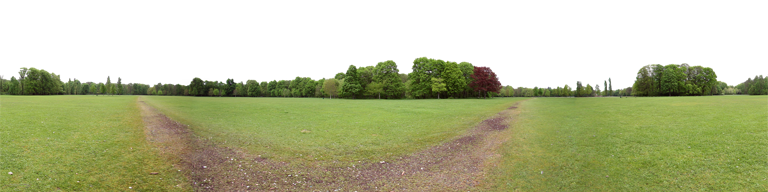
\includegraphics{egarden-narrow}
%\caption{Figure caption}
\end{figure}

I made the egarden into a 4096 x 1024 quite easily because there was a
lot of blank space above the horizon. This would allow 4 panels 1024 x
1024 pixels.in fact if I had a 8192 x 4096 panorama I could have made it
into 8 1024 x 1024 panels. This would have given me quite a high
resolution horizon

\begin{figure}[h]
\centering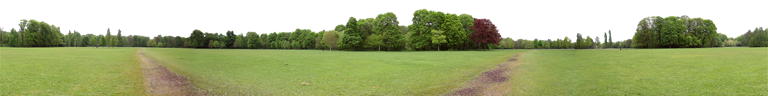
\includegraphics{egarden-narrow-2}
%\caption{Figure caption}
\end{figure}


\begin{enumerate}
\item
  Load the sections into TheGimp and process them into 1024 x 1024
  textures with alpha layers as before.
\item
  Next use a 2048 x 1024 version of the panorama in Stellarium. Drag the
  screen around so it produces a centralised picture on the Stellarium
  screen of the ground at the highest resolution possible and take a
  screen shot. This screen shot can be then processed into a quite
  effective ground texture in TheGimp that can be adjusted to match the
  rest of the panorama.
  \begin{figure}[h]
  \centering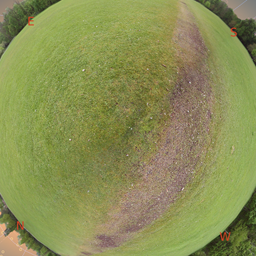
\includegraphics[scale=2.0]{egardembase}
  %\caption{Figure caption}
  \end{figure}
\item
  Make a new directory etc. for the landscape.
\item
  You can make it fit using the variablein the landscape.ini file
  decor\_alt\_angle=xx decor\_angle\_shift=xx and
  decor\_angle\_rotatez=xx.Then the ground can be matched with
  ground\_angle\_shift=xx and ground\_angle\_rotatez=xx.
\item
  Make sure the draw\_ground\_first=1 to ensure that the main panorama
  overplays the ground
\end{enumerate}

After re-starting Stellarium, your landscape will appear in the
landscape tab of the main menu, and can be selected as required.

When the panorama is finished it will be in *.jpg format. It will need
to be converted to a *.png with transparent background (alpha layer) and
have the sky removed. This is done in TheGimp as in the multipanel type.
When the sky is removed make sure you save the landscape in *.png
format.

The drawback with the spherical panorama is that few computer video
cards will reproduce a panorama larger than 4096 x 2048 pixels in
Stellarium and many will not do better than 2048 x 1024 pixels.

My computer will only do 2048 by 1024, If I try to load a larger type I
just get a white screen. With this problem I used the following
procedure to make the spherical into a four panel multi panel landscape
with a very effective ground that matched well.

\section{Making a Fish eye Panorama}
\label{making-a-fish-eye-panorama}

This sort of panorama needs a very expensive fisheye lens on your
camera. It is really only practical for a planetarium display to give a
simple more or less silouette landscape where the ground is completely
obscured. It can only be used with quite small pictures of no more than
1024 x 1024 pixels. Once you have your fisheye texture it must still be
processed in TheGimp to remove the sky and convert into an alpha layer
texture

\begin{figure}[h]
\centering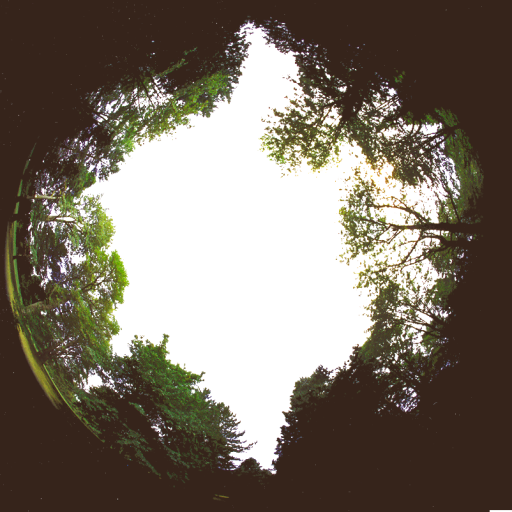
\includegraphics[scale=3.0]{trees_512}
%\caption{Figure caption}
\end{figure}

The sample supplied with Stellarium is called trees. The horizon needs
to be identified and the picture sized so that the panorama above the
horizon is sited to be about 80\% of the total extent and the the
balance of the border filled with a dark colour right up to the horizon.
This will make the horizon in your landscape at 0 degrees.

It is possible to make a synthetic fisheye texture using the same method
as making a ground from a spherical panorama but it is hardly worth the
trouble as even a simple 2048 x 1024 pixel sperical will give a far
better result.

%%% Local Variables: 
%%% mode: latex
%%% TeX-master: "guide"
%%% End: 
